% Created by tikzDevice version 0.10.1 on 2017-11-15 12:08:52
% !TEX encoding = UTF-8 Unicode
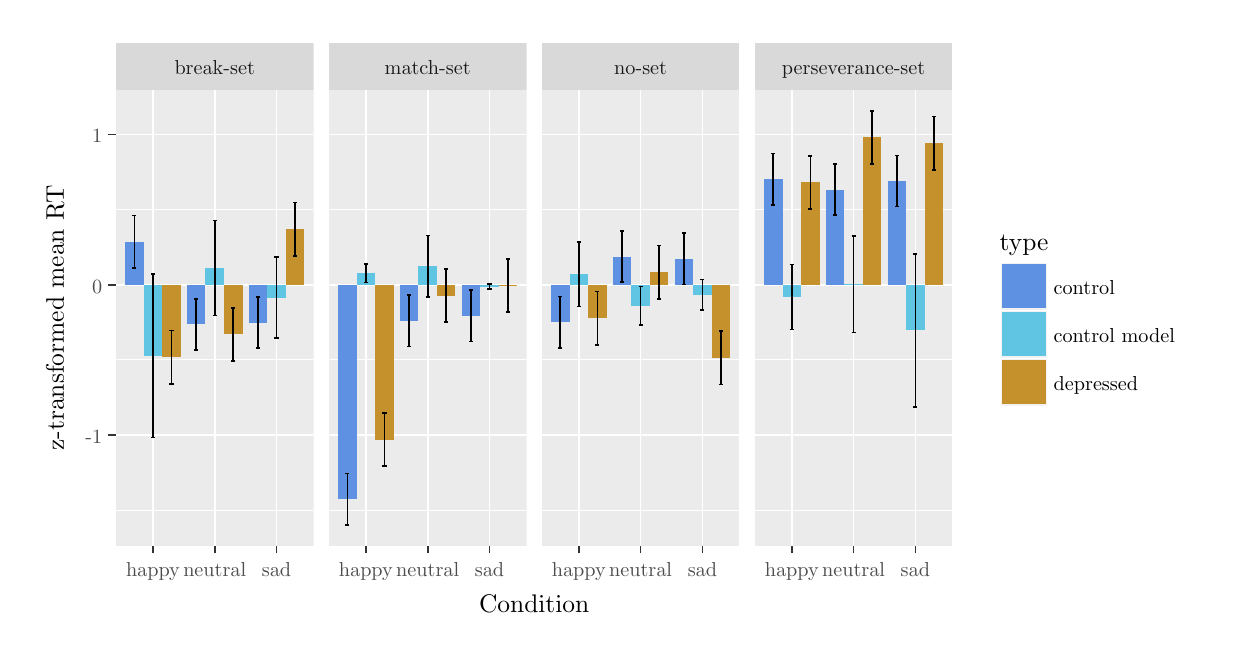
\begin{tikzpicture}[x=1pt,y=1pt]
\definecolor{fillColor}{RGB}{255,255,255}
\path[use as bounding box,fill=fillColor,fill opacity=0.00] (0,0) rectangle (433.62,216.81);
\begin{scope}
\path[clip] (  0.00,  0.00) rectangle (433.62,216.81);
\definecolor{drawColor}{RGB}{255,255,255}
\definecolor{fillColor}{RGB}{255,255,255}

\path[draw=drawColor,line width= 0.6pt,line join=round,line cap=round,fill=fillColor] (  0.00,  0.00) rectangle (433.62,216.81);
\end{scope}
\begin{scope}
\path[clip] ( 31.87, 29.59) rectangle (103.32,194.25);
\definecolor{fillColor}{gray}{0.92}

\path[fill=fillColor] ( 31.87, 29.59) rectangle (103.32,194.25);
\definecolor{drawColor}{RGB}{255,255,255}

\path[draw=drawColor,line width= 0.3pt,line join=round] ( 31.87, 42.48) --
	(103.32, 42.48);

\path[draw=drawColor,line width= 0.3pt,line join=round] ( 31.87, 96.76) --
	(103.32, 96.76);

\path[draw=drawColor,line width= 0.3pt,line join=round] ( 31.87,151.03) --
	(103.32,151.03);

\path[draw=drawColor,line width= 0.6pt,line join=round] ( 31.87, 69.62) --
	(103.32, 69.62);

\path[draw=drawColor,line width= 0.6pt,line join=round] ( 31.87,123.90) --
	(103.32,123.90);

\path[draw=drawColor,line width= 0.6pt,line join=round] ( 31.87,178.17) --
	(103.32,178.17);

\path[draw=drawColor,line width= 0.6pt,line join=round] ( 45.27, 29.59) --
	( 45.27,194.25);

\path[draw=drawColor,line width= 0.6pt,line join=round] ( 67.59, 29.59) --
	( 67.59,194.25);

\path[draw=drawColor,line width= 0.6pt,line join=round] ( 89.92, 29.59) --
	( 89.92,194.25);
\definecolor{fillColor}{RGB}{196,145,45}

\path[fill=fillColor] ( 48.62, 97.73) rectangle ( 55.31,123.90);
\definecolor{fillColor}{RGB}{95,197,226}

\path[fill=fillColor] ( 41.92, 98.24) rectangle ( 48.62,123.90);
\definecolor{fillColor}{RGB}{95,145,226}

\path[fill=fillColor] ( 35.22,123.90) rectangle ( 41.92,139.47);
\definecolor{fillColor}{RGB}{196,145,45}

\path[fill=fillColor] ( 70.94,105.98) rectangle ( 77.64,123.90);
\definecolor{fillColor}{RGB}{95,197,226}

\path[fill=fillColor] ( 64.25,123.90) rectangle ( 70.94,129.95);
\definecolor{fillColor}{RGB}{95,145,226}

\path[fill=fillColor] ( 57.55,109.61) rectangle ( 64.25,123.90);
\definecolor{fillColor}{RGB}{196,145,45}

\path[fill=fillColor] ( 93.27,123.90) rectangle ( 99.97,144.03);
\definecolor{fillColor}{RGB}{95,197,226}

\path[fill=fillColor] ( 86.57,119.24) rectangle ( 93.27,123.90);
\definecolor{fillColor}{RGB}{95,145,226}

\path[fill=fillColor] ( 79.87,110.23) rectangle ( 86.57,123.90);
\definecolor{drawColor}{RGB}{0,0,0}

\path[draw=drawColor,line width= 0.6pt,line join=round] ( 51.22,107.36) --
	( 52.71,107.36);

\path[draw=drawColor,line width= 0.6pt,line join=round] ( 51.97,107.36) --
	( 51.97, 88.09);

\path[draw=drawColor,line width= 0.6pt,line join=round] ( 51.22, 88.09) --
	( 52.71, 88.09);

\path[draw=drawColor,line width= 0.6pt,line join=round] ( 44.52,127.78) --
	( 46.01,127.78);

\path[draw=drawColor,line width= 0.6pt,line join=round] ( 45.27,127.78) --
	( 45.27, 68.70);

\path[draw=drawColor,line width= 0.6pt,line join=round] ( 44.52, 68.70) --
	( 46.01, 68.70);

\path[draw=drawColor,line width= 0.6pt,line join=round] ( 37.83,148.99) --
	( 39.31,148.99);

\path[draw=drawColor,line width= 0.6pt,line join=round] ( 38.57,148.99) --
	( 38.57,129.96);

\path[draw=drawColor,line width= 0.6pt,line join=round] ( 37.83,129.96) --
	( 39.31,129.96);

\path[draw=drawColor,line width= 0.6pt,line join=round] ( 73.55,115.58) --
	( 75.04,115.58);

\path[draw=drawColor,line width= 0.6pt,line join=round] ( 74.29,115.58) --
	( 74.29, 96.37);

\path[draw=drawColor,line width= 0.6pt,line join=round] ( 73.55, 96.37) --
	( 75.04, 96.37);

\path[draw=drawColor,line width= 0.6pt,line join=round] ( 66.85,147.09) --
	( 68.34,147.09);

\path[draw=drawColor,line width= 0.6pt,line join=round] ( 67.59,147.09) --
	( 67.59,112.81);

\path[draw=drawColor,line width= 0.6pt,line join=round] ( 66.85,112.81) --
	( 68.34,112.81);

\path[draw=drawColor,line width= 0.6pt,line join=round] ( 60.15,118.88) --
	( 61.64,118.88);

\path[draw=drawColor,line width= 0.6pt,line join=round] ( 60.90,118.88) --
	( 60.90,100.34);

\path[draw=drawColor,line width= 0.6pt,line join=round] ( 60.15,100.34) --
	( 61.64,100.34);

\path[draw=drawColor,line width= 0.6pt,line join=round] ( 95.88,153.67) --
	( 97.36,153.67);

\path[draw=drawColor,line width= 0.6pt,line join=round] ( 96.62,153.67) --
	( 96.62,134.40);

\path[draw=drawColor,line width= 0.6pt,line join=round] ( 95.88,134.40) --
	( 97.36,134.40);

\path[draw=drawColor,line width= 0.6pt,line join=round] ( 89.18,133.87) --
	( 90.67,133.87);

\path[draw=drawColor,line width= 0.6pt,line join=round] ( 89.92,133.87) --
	( 89.92,104.60);

\path[draw=drawColor,line width= 0.6pt,line join=round] ( 89.18,104.60) --
	( 90.67,104.60);

\path[draw=drawColor,line width= 0.6pt,line join=round] ( 82.48,119.50) --
	( 83.97,119.50);

\path[draw=drawColor,line width= 0.6pt,line join=round] ( 83.22,119.50) --
	( 83.22,100.96);

\path[draw=drawColor,line width= 0.6pt,line join=round] ( 82.48,100.96) --
	( 83.97,100.96);
\end{scope}
\begin{scope}
\path[clip] (108.82, 29.59) rectangle (180.27,194.25);
\definecolor{fillColor}{gray}{0.92}

\path[fill=fillColor] (108.82, 29.59) rectangle (180.27,194.25);
\definecolor{drawColor}{RGB}{255,255,255}

\path[draw=drawColor,line width= 0.3pt,line join=round] (108.82, 42.48) --
	(180.27, 42.48);

\path[draw=drawColor,line width= 0.3pt,line join=round] (108.82, 96.76) --
	(180.27, 96.76);

\path[draw=drawColor,line width= 0.3pt,line join=round] (108.82,151.03) --
	(180.27,151.03);

\path[draw=drawColor,line width= 0.6pt,line join=round] (108.82, 69.62) --
	(180.27, 69.62);

\path[draw=drawColor,line width= 0.6pt,line join=round] (108.82,123.90) --
	(180.27,123.90);

\path[draw=drawColor,line width= 0.6pt,line join=round] (108.82,178.17) --
	(180.27,178.17);

\path[draw=drawColor,line width= 0.6pt,line join=round] (122.21, 29.59) --
	(122.21,194.25);

\path[draw=drawColor,line width= 0.6pt,line join=round] (144.54, 29.59) --
	(144.54,194.25);

\path[draw=drawColor,line width= 0.6pt,line join=round] (166.87, 29.59) --
	(166.87,194.25);
\definecolor{fillColor}{RGB}{196,145,45}

\path[fill=fillColor] (125.56, 67.99) rectangle (132.26,123.90);
\definecolor{fillColor}{RGB}{95,197,226}

\path[fill=fillColor] (118.87,123.90) rectangle (125.56,128.06);
\definecolor{fillColor}{RGB}{95,145,226}

\path[fill=fillColor] (112.17, 46.37) rectangle (118.87,123.90);
\definecolor{fillColor}{RGB}{196,145,45}

\path[fill=fillColor] (147.89,119.96) rectangle (154.59,123.90);
\definecolor{fillColor}{RGB}{95,197,226}

\path[fill=fillColor] (141.19,123.90) rectangle (147.89,130.58);
\definecolor{fillColor}{RGB}{95,145,226}

\path[fill=fillColor] (134.49,110.90) rectangle (141.19,123.90);
\definecolor{fillColor}{RGB}{196,145,45}

\path[fill=fillColor] (170.22,123.71) rectangle (176.92,123.90);
\definecolor{fillColor}{RGB}{95,197,226}

\path[fill=fillColor] (163.52,123.21) rectangle (170.22,123.90);
\definecolor{fillColor}{RGB}{95,145,226}

\path[fill=fillColor] (156.82,112.69) rectangle (163.52,123.90);
\definecolor{drawColor}{RGB}{0,0,0}

\path[draw=drawColor,line width= 0.6pt,line join=round] (128.17, 77.59) --
	(129.66, 77.59);

\path[draw=drawColor,line width= 0.6pt,line join=round] (128.91, 77.59) --
	(128.91, 58.38);

\path[draw=drawColor,line width= 0.6pt,line join=round] (128.17, 58.38) --
	(129.66, 58.38);

\path[draw=drawColor,line width= 0.6pt,line join=round] (121.47,131.35) --
	(122.96,131.35);

\path[draw=drawColor,line width= 0.6pt,line join=round] (122.21,131.35) --
	(122.21,124.78);

\path[draw=drawColor,line width= 0.6pt,line join=round] (121.47,124.78) --
	(122.96,124.78);

\path[draw=drawColor,line width= 0.6pt,line join=round] (114.77, 55.67) --
	(116.26, 55.67);

\path[draw=drawColor,line width= 0.6pt,line join=round] (115.52, 55.67) --
	(115.52, 37.07);

\path[draw=drawColor,line width= 0.6pt,line join=round] (114.77, 37.07) --
	(116.26, 37.07);

\path[draw=drawColor,line width= 0.6pt,line join=round] (150.50,129.56) --
	(151.98,129.56);

\path[draw=drawColor,line width= 0.6pt,line join=round] (151.24,129.56) --
	(151.24,110.35);

\path[draw=drawColor,line width= 0.6pt,line join=round] (150.50,110.35) --
	(151.98,110.35);

\path[draw=drawColor,line width= 0.6pt,line join=round] (143.80,141.67) --
	(145.29,141.67);

\path[draw=drawColor,line width= 0.6pt,line join=round] (144.54,141.67) --
	(144.54,119.48);

\path[draw=drawColor,line width= 0.6pt,line join=round] (143.80,119.48) --
	(145.29,119.48);

\path[draw=drawColor,line width= 0.6pt,line join=round] (137.10,120.17) --
	(138.59,120.17);

\path[draw=drawColor,line width= 0.6pt,line join=round] (137.84,120.17) --
	(137.84,101.64);

\path[draw=drawColor,line width= 0.6pt,line join=round] (137.10,101.64) --
	(138.59,101.64);

\path[draw=drawColor,line width= 0.6pt,line join=round] (172.82,133.31) --
	(174.31,133.31);

\path[draw=drawColor,line width= 0.6pt,line join=round] (173.57,133.31) --
	(173.57,114.10);

\path[draw=drawColor,line width= 0.6pt,line join=round] (172.82,114.10) --
	(174.31,114.10);

\path[draw=drawColor,line width= 0.6pt,line join=round] (166.12,124.14) --
	(167.61,124.14);

\path[draw=drawColor,line width= 0.6pt,line join=round] (166.87,124.14) --
	(166.87,122.27);

\path[draw=drawColor,line width= 0.6pt,line join=round] (166.12,122.27) --
	(167.61,122.27);

\path[draw=drawColor,line width= 0.6pt,line join=round] (159.43,121.96) --
	(160.92,121.96);

\path[draw=drawColor,line width= 0.6pt,line join=round] (160.17,121.96) --
	(160.17,103.42);

\path[draw=drawColor,line width= 0.6pt,line join=round] (159.43,103.42) --
	(160.92,103.42);
\end{scope}
\begin{scope}
\path[clip] (185.77, 29.59) rectangle (257.21,194.25);
\definecolor{fillColor}{gray}{0.92}

\path[fill=fillColor] (185.77, 29.59) rectangle (257.21,194.25);
\definecolor{drawColor}{RGB}{255,255,255}

\path[draw=drawColor,line width= 0.3pt,line join=round] (185.77, 42.48) --
	(257.21, 42.48);

\path[draw=drawColor,line width= 0.3pt,line join=round] (185.77, 96.76) --
	(257.21, 96.76);

\path[draw=drawColor,line width= 0.3pt,line join=round] (185.77,151.03) --
	(257.21,151.03);

\path[draw=drawColor,line width= 0.6pt,line join=round] (185.77, 69.62) --
	(257.21, 69.62);

\path[draw=drawColor,line width= 0.6pt,line join=round] (185.77,123.90) --
	(257.21,123.90);

\path[draw=drawColor,line width= 0.6pt,line join=round] (185.77,178.17) --
	(257.21,178.17);

\path[draw=drawColor,line width= 0.6pt,line join=round] (199.16, 29.59) --
	(199.16,194.25);

\path[draw=drawColor,line width= 0.6pt,line join=round] (221.49, 29.59) --
	(221.49,194.25);

\path[draw=drawColor,line width= 0.6pt,line join=round] (243.82, 29.59) --
	(243.82,194.25);
\definecolor{fillColor}{RGB}{196,145,45}

\path[fill=fillColor] (202.51,111.83) rectangle (209.21,123.90);
\definecolor{fillColor}{RGB}{95,197,226}

\path[fill=fillColor] (195.81,123.90) rectangle (202.51,127.73);
\definecolor{fillColor}{RGB}{95,145,226}

\path[fill=fillColor] (189.11,110.41) rectangle (195.81,123.90);
\definecolor{fillColor}{RGB}{196,145,45}

\path[fill=fillColor] (224.84,123.90) rectangle (231.54,128.45);
\definecolor{fillColor}{RGB}{95,197,226}

\path[fill=fillColor] (218.14,116.30) rectangle (224.84,123.90);
\definecolor{fillColor}{RGB}{95,145,226}

\path[fill=fillColor] (211.44,123.90) rectangle (218.14,134.12);
\definecolor{fillColor}{RGB}{196,145,45}

\path[fill=fillColor] (247.17, 97.54) rectangle (253.86,123.90);
\definecolor{fillColor}{RGB}{95,197,226}

\path[fill=fillColor] (240.47,120.30) rectangle (247.17,123.90);
\definecolor{fillColor}{RGB}{95,145,226}

\path[fill=fillColor] (233.77,123.90) rectangle (240.47,133.32);
\definecolor{drawColor}{RGB}{0,0,0}

\path[draw=drawColor,line width= 0.6pt,line join=round] (205.12,121.43) --
	(206.60,121.43);

\path[draw=drawColor,line width= 0.6pt,line join=round] (205.86,121.43) --
	(205.86,102.22);

\path[draw=drawColor,line width= 0.6pt,line join=round] (205.12,102.22) --
	(206.60,102.22);

\path[draw=drawColor,line width= 0.6pt,line join=round] (198.42,139.42) --
	(199.91,139.42);

\path[draw=drawColor,line width= 0.6pt,line join=round] (199.16,139.42) --
	(199.16,116.05);

\path[draw=drawColor,line width= 0.6pt,line join=round] (198.42,116.05) --
	(199.91,116.05);

\path[draw=drawColor,line width= 0.6pt,line join=round] (191.72,119.71) --
	(193.21,119.71);

\path[draw=drawColor,line width= 0.6pt,line join=round] (192.46,119.71) --
	(192.46,101.11);

\path[draw=drawColor,line width= 0.6pt,line join=round] (191.72,101.11) --
	(193.21,101.11);

\path[draw=drawColor,line width= 0.6pt,line join=round] (227.44,138.09) --
	(228.93,138.09);

\path[draw=drawColor,line width= 0.6pt,line join=round] (228.19,138.09) --
	(228.19,118.82);

\path[draw=drawColor,line width= 0.6pt,line join=round] (227.44,118.82) --
	(228.93,118.82);

\path[draw=drawColor,line width= 0.6pt,line join=round] (220.74,123.28) --
	(222.23,123.28);

\path[draw=drawColor,line width= 0.6pt,line join=round] (221.49,123.28) --
	(221.49,109.32);

\path[draw=drawColor,line width= 0.6pt,line join=round] (220.74,109.32) --
	(222.23,109.32);

\path[draw=drawColor,line width= 0.6pt,line join=round] (214.05,143.39) --
	(215.53,143.39);

\path[draw=drawColor,line width= 0.6pt,line join=round] (214.79,143.39) --
	(214.79,124.85);

\path[draw=drawColor,line width= 0.6pt,line join=round] (214.05,124.85) --
	(215.53,124.85);

\path[draw=drawColor,line width= 0.6pt,line join=round] (249.77,107.15) --
	(251.26,107.15);

\path[draw=drawColor,line width= 0.6pt,line join=round] (250.51,107.15) --
	(250.51, 87.93);

\path[draw=drawColor,line width= 0.6pt,line join=round] (249.77, 87.93) --
	(251.26, 87.93);

\path[draw=drawColor,line width= 0.6pt,line join=round] (243.07,125.80) --
	(244.56,125.80);

\path[draw=drawColor,line width= 0.6pt,line join=round] (243.82,125.80) --
	(243.82,114.79);

\path[draw=drawColor,line width= 0.6pt,line join=round] (243.07,114.79) --
	(244.56,114.79);

\path[draw=drawColor,line width= 0.6pt,line join=round] (236.37,142.58) --
	(237.86,142.58);

\path[draw=drawColor,line width= 0.6pt,line join=round] (237.12,142.58) --
	(237.12,124.05);

\path[draw=drawColor,line width= 0.6pt,line join=round] (236.37,124.05) --
	(237.86,124.05);
\end{scope}
\begin{scope}
\path[clip] (262.71, 29.59) rectangle (334.16,194.25);
\definecolor{fillColor}{gray}{0.92}

\path[fill=fillColor] (262.71, 29.59) rectangle (334.16,194.25);
\definecolor{drawColor}{RGB}{255,255,255}

\path[draw=drawColor,line width= 0.3pt,line join=round] (262.71, 42.48) --
	(334.16, 42.48);

\path[draw=drawColor,line width= 0.3pt,line join=round] (262.71, 96.76) --
	(334.16, 96.76);

\path[draw=drawColor,line width= 0.3pt,line join=round] (262.71,151.03) --
	(334.16,151.03);

\path[draw=drawColor,line width= 0.6pt,line join=round] (262.71, 69.62) --
	(334.16, 69.62);

\path[draw=drawColor,line width= 0.6pt,line join=round] (262.71,123.90) --
	(334.16,123.90);

\path[draw=drawColor,line width= 0.6pt,line join=round] (262.71,178.17) --
	(334.16,178.17);

\path[draw=drawColor,line width= 0.6pt,line join=round] (276.11, 29.59) --
	(276.11,194.25);

\path[draw=drawColor,line width= 0.6pt,line join=round] (298.44, 29.59) --
	(298.44,194.25);

\path[draw=drawColor,line width= 0.6pt,line join=round] (320.76, 29.59) --
	(320.76,194.25);
\definecolor{fillColor}{RGB}{196,145,45}

\path[fill=fillColor] (279.46,123.90) rectangle (286.16,160.90);
\definecolor{fillColor}{RGB}{95,197,226}

\path[fill=fillColor] (272.76,119.45) rectangle (279.46,123.90);
\definecolor{fillColor}{RGB}{95,145,226}

\path[fill=fillColor] (266.06,123.90) rectangle (272.76,162.07);
\definecolor{fillColor}{RGB}{196,145,45}

\path[fill=fillColor] (301.78,123.90) rectangle (308.48,177.16);
\definecolor{fillColor}{RGB}{95,197,226}

\path[fill=fillColor] (295.09,123.90) rectangle (301.78,124.13);
\definecolor{fillColor}{RGB}{95,145,226}

\path[fill=fillColor] (288.39,123.90) rectangle (295.09,158.32);
\definecolor{fillColor}{RGB}{196,145,45}

\path[fill=fillColor] (324.11,123.90) rectangle (330.81,175.07);
\definecolor{fillColor}{RGB}{95,197,226}

\path[fill=fillColor] (317.41,107.41) rectangle (324.11,123.90);
\definecolor{fillColor}{RGB}{95,145,226}

\path[fill=fillColor] (310.72,123.90) rectangle (317.41,161.39);
\definecolor{drawColor}{RGB}{0,0,0}

\path[draw=drawColor,line width= 0.6pt,line join=round] (282.06,170.51) --
	(283.55,170.51);

\path[draw=drawColor,line width= 0.6pt,line join=round] (282.81,170.51) --
	(282.81,151.30);

\path[draw=drawColor,line width= 0.6pt,line join=round] (282.06,151.30) --
	(283.55,151.30);

\path[draw=drawColor,line width= 0.6pt,line join=round] (275.36,131.20) --
	(276.85,131.20);

\path[draw=drawColor,line width= 0.6pt,line join=round] (276.11,131.20) --
	(276.11,107.70);

\path[draw=drawColor,line width= 0.6pt,line join=round] (275.36,107.70) --
	(276.85,107.70);

\path[draw=drawColor,line width= 0.6pt,line join=round] (268.67,171.34) --
	(270.15,171.34);

\path[draw=drawColor,line width= 0.6pt,line join=round] (269.41,171.34) --
	(269.41,152.80);

\path[draw=drawColor,line width= 0.6pt,line join=round] (268.67,152.80) --
	(270.15,152.80);

\path[draw=drawColor,line width= 0.6pt,line join=round] (304.39,186.76) --
	(305.88,186.76);

\path[draw=drawColor,line width= 0.6pt,line join=round] (305.13,186.76) --
	(305.13,167.55);

\path[draw=drawColor,line width= 0.6pt,line join=round] (304.39,167.55) --
	(305.88,167.55);

\path[draw=drawColor,line width= 0.6pt,line join=round] (297.69,141.59) --
	(299.18,141.59);

\path[draw=drawColor,line width= 0.6pt,line join=round] (298.44,141.59) --
	(298.44,106.67);

\path[draw=drawColor,line width= 0.6pt,line join=round] (297.69,106.67) --
	(299.18,106.67);

\path[draw=drawColor,line width= 0.6pt,line join=round] (290.99,167.58) --
	(292.48,167.58);

\path[draw=drawColor,line width= 0.6pt,line join=round] (291.74,167.58) --
	(291.74,149.05);

\path[draw=drawColor,line width= 0.6pt,line join=round] (290.99,149.05) --
	(292.48,149.05);

\path[draw=drawColor,line width= 0.6pt,line join=round] (326.72,184.67) --
	(328.21,184.67);

\path[draw=drawColor,line width= 0.6pt,line join=round] (327.46,184.67) --
	(327.46,165.46);

\path[draw=drawColor,line width= 0.6pt,line join=round] (326.72,165.46) --
	(328.21,165.46);

\path[draw=drawColor,line width= 0.6pt,line join=round] (320.02,134.99) --
	(321.51,134.99);

\path[draw=drawColor,line width= 0.6pt,line join=round] (320.76,134.99) --
	(320.76, 79.83);

\path[draw=drawColor,line width= 0.6pt,line join=round] (320.02, 79.83) --
	(321.51, 79.83);

\path[draw=drawColor,line width= 0.6pt,line join=round] (313.32,170.66) --
	(314.81,170.66);

\path[draw=drawColor,line width= 0.6pt,line join=round] (314.06,170.66) --
	(314.06,152.13);

\path[draw=drawColor,line width= 0.6pt,line join=round] (313.32,152.13) --
	(314.81,152.13);
\end{scope}
\begin{scope}
\path[clip] ( 31.87,194.25) rectangle (103.32,211.31);
\definecolor{fillColor}{gray}{0.85}

\path[fill=fillColor] ( 31.87,194.25) rectangle (103.32,211.31);
\definecolor{drawColor}{gray}{0.10}

\node[text=drawColor,anchor=base,inner sep=0pt, outer sep=0pt, scale=  0.73] at ( 67.59,199.75) {break-set};
\end{scope}
\begin{scope}
\path[clip] (108.82,194.25) rectangle (180.27,211.31);
\definecolor{fillColor}{gray}{0.85}

\path[fill=fillColor] (108.82,194.25) rectangle (180.27,211.31);
\definecolor{drawColor}{gray}{0.10}

\node[text=drawColor,anchor=base,inner sep=0pt, outer sep=0pt, scale=  0.73] at (144.54,199.75) {match-set};
\end{scope}
\begin{scope}
\path[clip] (185.77,194.25) rectangle (257.21,211.31);
\definecolor{fillColor}{gray}{0.85}

\path[fill=fillColor] (185.77,194.25) rectangle (257.21,211.31);
\definecolor{drawColor}{gray}{0.10}

\node[text=drawColor,anchor=base,inner sep=0pt, outer sep=0pt, scale=  0.73] at (221.49,199.75) {no-set};
\end{scope}
\begin{scope}
\path[clip] (262.71,194.25) rectangle (334.16,211.31);
\definecolor{fillColor}{gray}{0.85}

\path[fill=fillColor] (262.71,194.25) rectangle (334.16,211.31);
\definecolor{drawColor}{gray}{0.10}

\node[text=drawColor,anchor=base,inner sep=0pt, outer sep=0pt, scale=  0.73] at (298.44,199.75) {perseverance-set};
\end{scope}
\begin{scope}
\path[clip] (  0.00,  0.00) rectangle (433.62,216.81);
\definecolor{drawColor}{gray}{0.20}

\path[draw=drawColor,line width= 0.6pt,line join=round] ( 45.27, 26.84) --
	( 45.27, 29.59);

\path[draw=drawColor,line width= 0.6pt,line join=round] ( 67.59, 26.84) --
	( 67.59, 29.59);

\path[draw=drawColor,line width= 0.6pt,line join=round] ( 89.92, 26.84) --
	( 89.92, 29.59);
\end{scope}
\begin{scope}
\path[clip] (  0.00,  0.00) rectangle (433.62,216.81);
\definecolor{drawColor}{gray}{0.30}

\node[text=drawColor,anchor=base,inner sep=0pt, outer sep=0pt, scale=  0.73] at ( 45.27, 18.58) {happy};

\node[text=drawColor,anchor=base,inner sep=0pt, outer sep=0pt, scale=  0.73] at ( 67.59, 18.58) {neutral};

\node[text=drawColor,anchor=base,inner sep=0pt, outer sep=0pt, scale=  0.73] at ( 89.92, 18.58) {sad};
\end{scope}
\begin{scope}
\path[clip] (  0.00,  0.00) rectangle (433.62,216.81);
\definecolor{drawColor}{gray}{0.20}

\path[draw=drawColor,line width= 0.6pt,line join=round] (122.21, 26.84) --
	(122.21, 29.59);

\path[draw=drawColor,line width= 0.6pt,line join=round] (144.54, 26.84) --
	(144.54, 29.59);

\path[draw=drawColor,line width= 0.6pt,line join=round] (166.87, 26.84) --
	(166.87, 29.59);
\end{scope}
\begin{scope}
\path[clip] (  0.00,  0.00) rectangle (433.62,216.81);
\definecolor{drawColor}{gray}{0.30}

\node[text=drawColor,anchor=base,inner sep=0pt, outer sep=0pt, scale=  0.73] at (122.21, 18.58) {happy};

\node[text=drawColor,anchor=base,inner sep=0pt, outer sep=0pt, scale=  0.73] at (144.54, 18.58) {neutral};

\node[text=drawColor,anchor=base,inner sep=0pt, outer sep=0pt, scale=  0.73] at (166.87, 18.58) {sad};
\end{scope}
\begin{scope}
\path[clip] (  0.00,  0.00) rectangle (433.62,216.81);
\definecolor{drawColor}{gray}{0.20}

\path[draw=drawColor,line width= 0.6pt,line join=round] (199.16, 26.84) --
	(199.16, 29.59);

\path[draw=drawColor,line width= 0.6pt,line join=round] (221.49, 26.84) --
	(221.49, 29.59);

\path[draw=drawColor,line width= 0.6pt,line join=round] (243.82, 26.84) --
	(243.82, 29.59);
\end{scope}
\begin{scope}
\path[clip] (  0.00,  0.00) rectangle (433.62,216.81);
\definecolor{drawColor}{gray}{0.30}

\node[text=drawColor,anchor=base,inner sep=0pt, outer sep=0pt, scale=  0.73] at (199.16, 18.58) {happy};

\node[text=drawColor,anchor=base,inner sep=0pt, outer sep=0pt, scale=  0.73] at (221.49, 18.58) {neutral};

\node[text=drawColor,anchor=base,inner sep=0pt, outer sep=0pt, scale=  0.73] at (243.82, 18.58) {sad};
\end{scope}
\begin{scope}
\path[clip] (  0.00,  0.00) rectangle (433.62,216.81);
\definecolor{drawColor}{gray}{0.20}

\path[draw=drawColor,line width= 0.6pt,line join=round] (276.11, 26.84) --
	(276.11, 29.59);

\path[draw=drawColor,line width= 0.6pt,line join=round] (298.44, 26.84) --
	(298.44, 29.59);

\path[draw=drawColor,line width= 0.6pt,line join=round] (320.76, 26.84) --
	(320.76, 29.59);
\end{scope}
\begin{scope}
\path[clip] (  0.00,  0.00) rectangle (433.62,216.81);
\definecolor{drawColor}{gray}{0.30}

\node[text=drawColor,anchor=base,inner sep=0pt, outer sep=0pt, scale=  0.73] at (276.11, 18.58) {happy};

\node[text=drawColor,anchor=base,inner sep=0pt, outer sep=0pt, scale=  0.73] at (298.44, 18.58) {neutral};

\node[text=drawColor,anchor=base,inner sep=0pt, outer sep=0pt, scale=  0.73] at (320.76, 18.58) {sad};
\end{scope}
\begin{scope}
\path[clip] (  0.00,  0.00) rectangle (433.62,216.81);
\definecolor{drawColor}{gray}{0.30}

\node[text=drawColor,anchor=base east,inner sep=0pt, outer sep=0pt, scale=  0.73] at ( 26.92, 66.59) {-1};

\node[text=drawColor,anchor=base east,inner sep=0pt, outer sep=0pt, scale=  0.73] at ( 26.92,120.87) {0};

\node[text=drawColor,anchor=base east,inner sep=0pt, outer sep=0pt, scale=  0.73] at ( 26.92,175.14) {1};
\end{scope}
\begin{scope}
\path[clip] (  0.00,  0.00) rectangle (433.62,216.81);
\definecolor{drawColor}{gray}{0.20}

\path[draw=drawColor,line width= 0.6pt,line join=round] ( 29.12, 69.62) --
	( 31.87, 69.62);

\path[draw=drawColor,line width= 0.6pt,line join=round] ( 29.12,123.90) --
	( 31.87,123.90);

\path[draw=drawColor,line width= 0.6pt,line join=round] ( 29.12,178.17) --
	( 31.87,178.17);
\end{scope}
\begin{scope}
\path[clip] (  0.00,  0.00) rectangle (433.62,216.81);
\definecolor{drawColor}{RGB}{0,0,0}

\node[text=drawColor,anchor=base,inner sep=0pt, outer sep=0pt, scale=  0.92] at (183.02,  5.50) {Condition};
\end{scope}
\begin{scope}
\path[clip] (  0.00,  0.00) rectangle (433.62,216.81);
\definecolor{drawColor}{RGB}{0,0,0}

\node[text=drawColor,rotate= 90.00,anchor=base,inner sep=0pt, outer sep=0pt, scale=  0.92] at ( 13.08,111.92) {z-transformed mean RT};
\end{scope}
\begin{scope}
\path[clip] (  0.00,  0.00) rectangle (433.62,216.81);
\definecolor{fillColor}{RGB}{255,255,255}

\path[fill=fillColor] (345.54, 74.25) rectangle (428.12,149.58);
\end{scope}
\begin{scope}
\path[clip] (  0.00,  0.00) rectangle (433.62,216.81);
\definecolor{drawColor}{RGB}{0,0,0}

\node[text=drawColor,anchor=base west,inner sep=0pt, outer sep=0pt, scale=  0.92] at (351.23,136.32) {type};
\end{scope}
\begin{scope}
\path[clip] (  0.00,  0.00) rectangle (433.62,216.81);
\definecolor{drawColor}{RGB}{255,255,255}
\definecolor{fillColor}{gray}{0.95}

\path[draw=drawColor,line width= 0.6pt,line join=round,line cap=round,fill=fillColor] (351.23,114.63) rectangle (368.58,131.98);
\end{scope}
\begin{scope}
\path[clip] (  0.00,  0.00) rectangle (433.62,216.81);
\definecolor{fillColor}{RGB}{95,145,226}

\path[fill=fillColor] (351.94,115.35) rectangle (367.86,131.27);
\end{scope}
\begin{scope}
\path[clip] (  0.00,  0.00) rectangle (433.62,216.81);
\definecolor{drawColor}{RGB}{255,255,255}
\definecolor{fillColor}{gray}{0.95}

\path[draw=drawColor,line width= 0.6pt,line join=round,line cap=round,fill=fillColor] (351.23, 97.29) rectangle (368.58,114.63);
\end{scope}
\begin{scope}
\path[clip] (  0.00,  0.00) rectangle (433.62,216.81);
\definecolor{fillColor}{RGB}{95,197,226}

\path[fill=fillColor] (351.94, 98.00) rectangle (367.86,113.92);
\end{scope}
\begin{scope}
\path[clip] (  0.00,  0.00) rectangle (433.62,216.81);
\definecolor{drawColor}{RGB}{255,255,255}
\definecolor{fillColor}{gray}{0.95}

\path[draw=drawColor,line width= 0.6pt,line join=round,line cap=round,fill=fillColor] (351.23, 79.94) rectangle (368.58, 97.29);
\end{scope}
\begin{scope}
\path[clip] (  0.00,  0.00) rectangle (433.62,216.81);
\definecolor{fillColor}{RGB}{196,145,45}

\path[fill=fillColor] (351.94, 80.66) rectangle (367.86, 96.58);
\end{scope}
\begin{scope}
\path[clip] (  0.00,  0.00) rectangle (433.62,216.81);
\definecolor{drawColor}{RGB}{0,0,0}

\node[text=drawColor,anchor=base west,inner sep=0pt, outer sep=0pt, scale=  0.73] at (370.74,120.28) {control};
\end{scope}
\begin{scope}
\path[clip] (  0.00,  0.00) rectangle (433.62,216.81);
\definecolor{drawColor}{RGB}{0,0,0}

\node[text=drawColor,anchor=base west,inner sep=0pt, outer sep=0pt, scale=  0.73] at (370.74,102.93) {control model};
\end{scope}
\begin{scope}
\path[clip] (  0.00,  0.00) rectangle (433.62,216.81);
\definecolor{drawColor}{RGB}{0,0,0}

\node[text=drawColor,anchor=base west,inner sep=0pt, outer sep=0pt, scale=  0.73] at (370.74, 85.59) {depressed};
\end{scope}
\end{tikzpicture}
